 \begin{center}\large\textbf{Readings: Chapter 8 (read 8.1-8.4)}\\
\normalsize \end{center}
\large ~\hrulefill
~\\
\normalsize

We now turn our focus back to comparing means from different populations.  In chapter 6, we saw how to compare the (true) means from two (roughly) normal populations (both with equal and unequal variance).\\~\\

We may however have interest in comparing the (true) means from more than two populations, say $t$ populations.  This type of question often comes up when conducting a completely randomized experiment (CRD).\\~\\

In a CRD we have $N$ total units (the book uses $n_T$ to represent this number).  We have $t$ treatments - recall a treatment is a specific experimental condition which, in an experiment, we assign to the experimental units.  This treatment may come from the levels of a single factor or the combinations of levels from several factors.\\~\\

Let $n_i$ denote the number of replicates for treatment i (i=1,...,t) (i.e. the \# of units assigned to that treatment).  In a balanced CRD design, we have $n_i=n$ for every treatment i.  Thus, the total number of units can be given by $N=nt$ (or in the book notation $n_T=nt$). \\~\\

The CRD design randomly assigns the treatments to the units (treating every unit as interchangeable).\\~\\

Therefore, we can consider having $t$ different populations that we now want to compare.  For instance, we may want to know if the means are equal for each population (or the standard deviations, medians, etc.)\\~\\
  
\newpage

Example:  (some description taken from Goosen, 2014)\\
Consider having 24 pieces of cheese.  Color of the cheese is important in terms of consumer satisfaction.  We have interest in how the color differs for 4 different types of corn syrup (26, 42, 55, and 62) (4 treatments).  A CRD design is decided upon and we randomly assign each corn syrup type to 6 pieces of cheese (6 replicates for each treatment).\\~\\
As a response, we measure the color using a 3 part CIE L*a*b* Color System.
\begin{itemize}
\item `L' reflects the lightness of a sample, from black (L = 0) to white (L = 100) and runs from top to bottom.
\item `a' defines the shades from red (positive values) to green (negative values). 
\item `b' defines the shades from yellow (positive values) to blue (negative values).
\end{itemize}
All three of these could be treated as responses (and analyzed together), but for our purposes we will only look at the `L' response variable.\\~\\
Again, we will focus on the means of the population.  How might we make inference here?\\~\\
Define
\begin{itemize}
\item $\mu_1$ = mean `L' score for \textbf{all} pieces of cheese that with corn syrup 26.
\item $\mu_2$ = mean `L' score for \textbf{all} pieces of cheese that with corn syrup 42.
\item $\mu_3$ = mean `L' score for \textbf{all} pieces of cheese that with corn syrup 55.
\item $\mu_4$ = mean `L' score for \textbf{all} pieces of cheese that with corn syrup 62.
\end{itemize}

We want to test the hypotheses
$$H_0: \mu_1=\mu_2=\mu_3=\mu_4~~~~vs~~~~H_A:\mbox{at least one mean differs}$$~\\

For two independent samples, we said if the samples came from normal populations with equal variance we could use 
$$T=\frac{\bar{Y}-\bar{X}}{\sqrt{S_p^2(1/n_1+1/n_2)}}~~~~\mbox{where}~~S_p^2 = \frac{(n_1-1)S_1^2+(n_2-1)S_2^2}{n_1+n_2-2}$$
as a test statistic to make our inference.  Now we have more than 2 populations, so this exact set-up won't work, but we can do something else.

\newpage

\Large ANOVA for analyzing a CRD \normalsize\\~\\
Data and labeling:  
\begin{center}
\begin{tabular}{cc|cc}
Corn Syrup & Replicate \# & `L' measurement  & Label\\\hline
26 &1& 51.89&$y_{11}$\\
26 &2& 51.52&$y_{12}$\\
26 &3& 52.69&$y_{13}$\\
26 &4& 52.06&$y_{14}$\\
26 &5& 51.63&$y_{15}$\\
26 &6& 52.73&$y_{16}$\\
42 &1& 47.21&$y_{21}$\\
42 &2& 48.57&$y_{22}$\\
42 &3& 47.57&$y_{23}$\\
42 &4& 46.85&$y_{24}$\\
42 &5& 48.64&$y_{25}$\\
42 &6& 47.49&$y_{26}$\\
55 &1& 41.43&$y_{31}$\\
55& 2& 42.31&$y_{32}$\\
55& 3& 42.31&$y_{33}$\\
55& 4& 41.49&$y_{34}$\\
55& 5& 42.12&$y_{35}$\\
55& 6& 42.65&$y_{36}$\\
62 &1& 45.99&$y_{41}$\\
62 &2& 46.66&$y_{42}$\\
62 &3& 47.35&$y_{43}$\\
62 &4& 45.83&$y_{44}$\\
62 &5& 46.77&$y_{45}$\\
62 &6& 47.88&$y_{46}$\\
\end{tabular}
\end{center}

We now need two subscripts to represent which observation we are talking about. The first subscript (i) represents the treatment group, where as the second subscript (j) represent the replicate number.\\~\\

Consider the following two hypothetical set of boxplots for this data.  Which would give evidence that the (true) means differ?
\begin{center}
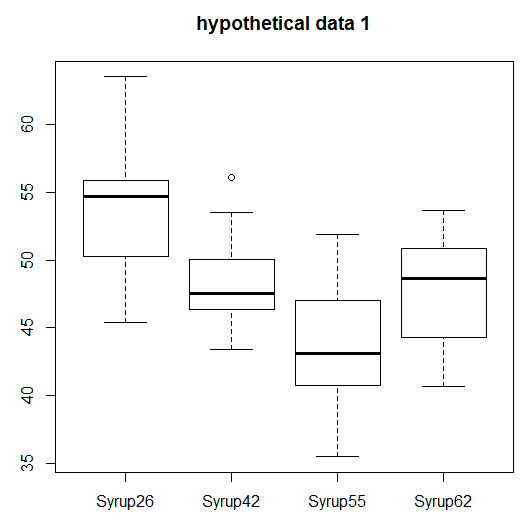
\includegraphics[scale=0.4]{fakebox1}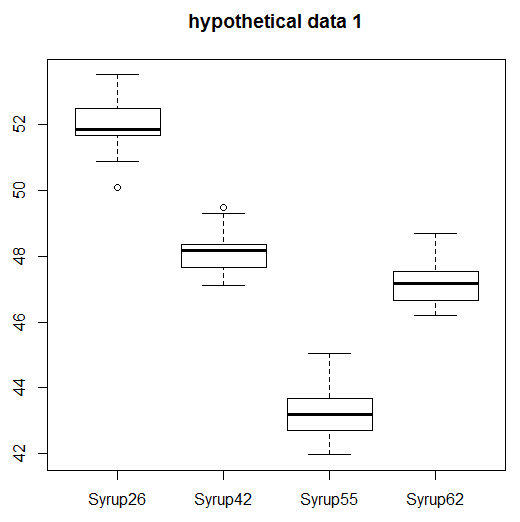
\includegraphics[scale=0.4]{fakebox2}
\end{center}

\newpage

\Large ANOVA = Analysis of Variance\normalsize\\~\\
In this case, compare variation `within' groups to variation `between' groups.\\~\\
Assumptions: 
$$Y_{1j}\sim^{iid}N(\mu_1,\sigma^2)$$
$$Y_{2j}\sim^{iid}N(\mu_2,\sigma^2)$$
$$Y_{3j}\sim^{iid}N(\mu_3,\sigma^2)$$
$$Y_{4j}\sim^{iid}N(\mu_4,\sigma^2)$$
and each sample is independent of one another.  \\~\\
That is, the populations are independent random samples from normally distributed parent populations with equal variances.  Rather than write this all out we will just say
$$Y_{ij}\sim^{iid}N(\mu_i,\sigma^2)$$

\begin{wrapfigure}{r}{0.5\textwidth}
  \begin{center}
    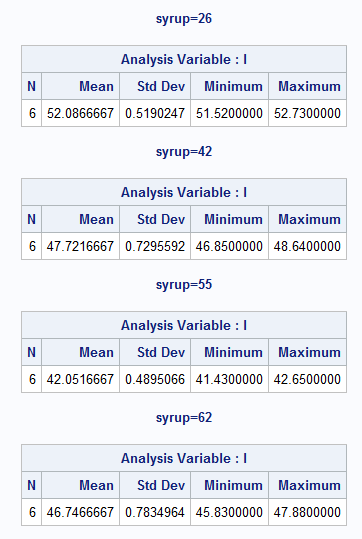
\includegraphics[width=0.48\textwidth]{colorsummary}
  \end{center}
  \caption{summary from proc means. - 
	proc means data=cheese;
  by syrup; var L; run;}
\end{wrapfigure}

\large \textbf{Within group variation} \normalsize\\
In two samples, to estimate the common variance $\sigma^2$ we used $S_p^2$.  Here we use the same exact idea:
$$MS(E) = MS(W) = S^2_w $$
$$=\frac{(n_1-1)S^2_1+(n_2-1)S^2_2+...+(n_t-1)S^2_t}{n_1+n_2+...+n_t-t}$$
For a balanced design we have
$$MS(E) = MS(W) = S^2_w = \frac{(n-1)(S^2_1+...+S^2_t)}{N-t} $$
$$= \frac{(n-1)(S^2_1+...+S^2_t)}{nt-t}=\frac{S^2_1+...+S^2_t}{t}$$
(i.e. just the simple average of the variances).\\~\\
With the double subscript our formula for $S^2_i$ is given by 
$$S^2_i = \frac{\sum_{j=1}^{n}(Y_{ij}-\bar{Y}_{i\bullet})^2}{n-1}$$
where the group mean $\bar{Y}_{i\bullet}$ is given by
$$\bar{Y}_{i\bullet} = \frac{\sum_{j=1}^{n}Y_{ij}}{n}$$
Thus, for a balanced design $MS(E)$ is written 
\begin{flushleft}
$MS(E)=\frac{\sum_{i=1}^{t}\sum_{j=1}^{n}(Y_{ij}-\bar{Y}_{i\bullet})^2}{t(n-1)}$
\end{flushleft}

\begin{wrapfigure}{r}{0.5\textwidth}
	\begin{center}
		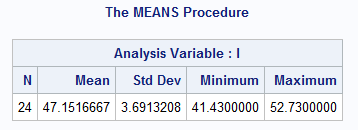
\includegraphics[width=0.48\textwidth]{colorsum}
  \end{center}
  \caption{summary from proc means
	proc means data=cheese;
var L; run;}
\end{wrapfigure}

\large \textbf{Between group variation} \normalsize\\
Variation between groups is judged by the variation between the group means:
$$MS(T) = MS(B) = S^2_b = \frac{\sum_{i=1}^{t}\sum_{j=1}^{n}(\bar{Y}_{i\bullet}-\bar{Y}_{\bullet\bullet})^2}{t-1}$$
where $\bar{Y}_{\bullet\bullet}$ is the overall mean 
$$\bar{Y}_{\bullet\bullet}=\frac{\sum_{i=1}^{t}\sum_{j=1}^{n}Y_{ij}}{nt}$$
~\\
\begin{flushright}
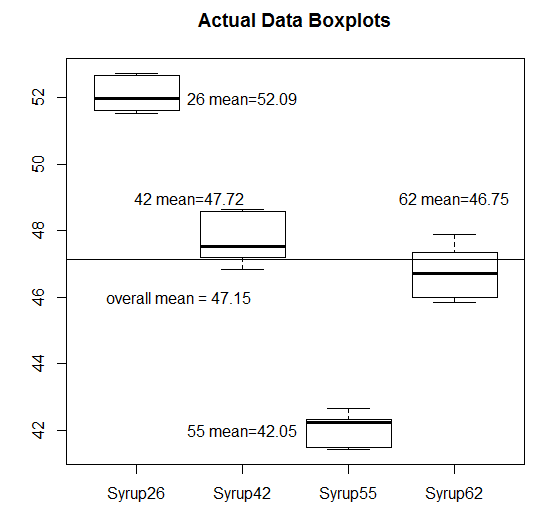
\includegraphics[scale=0.7]{colorboxplot}
\end{flushright}

For our hypotheses:
$$H_0: \mu_1=\mu_2=\mu_3=\mu_4~~~~vs~~~~H_A:\mbox{at least one mean differs}$$
Test statistic is:
$$F=\frac{MS(T)}{MS(E)}=\frac{S^2_b}{S^2_w}\sim F_{t-1,N-t}$$
We reject $H_0$ for large values of $F$, values greater than $F_{t-l,N-t,\alpha}$.\\~\\
We get a p-value by $P(F_{t-1,N-t}>F_{obs})$.

\newpage

To get this analysis in SAS we can run the code:\\
\begin{verbatim}
proc anova data=cheese;
      class syrup;
      model L = syrup;
      means syrup/tukey;
run;
\end{verbatim}

\begin{flushleft}
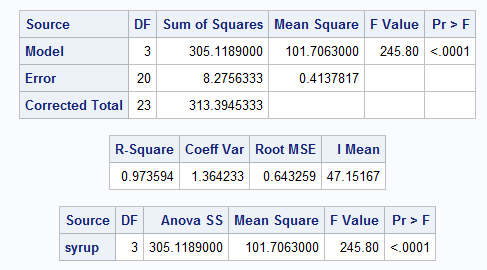
\includegraphics[scale=0.85]{coloranova1}\\
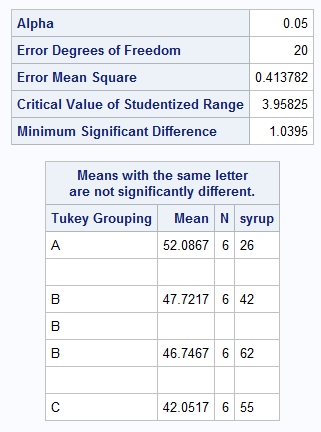
\includegraphics[scale=0.85]{coloranova2}
\end{flushleft}

\newpage

\Large How do we view the ANOVA `model'?\normalsize \\
We made the assumption that $Y_{ij}\sim^{iid}N(\mu_{i},\sigma^2)$.  Instead of viewing it in this form, we look at it as
$$Y_{ij}=\mu_{i}+E_{ij}$$
where $E_{ij}\sim^{iid}N(0,\sigma^2)$.  So for $i=1$ we have
$$Y_{1j}=\mu_{1}+E_{1j}$$
which is adding the constant $\mu_1$ to the $N(0,\sigma^2)$ distribution, giving $Y_{1j}\sim^{iid}N(\mu_{1},\sigma^2)$.\\~\\~\\

Usually we then change this to a different parameterization -
$$Y_{ij}=\mu+\tau_{i}+E_{ij}$$
where $\mu$ is the overall (grand) mean, $\tau_i$ is the effect for the $i^{th}$ treatment, and $E_{ij}\sim^{iid}N(0,\sigma^2)$.\\~\\
So for $i=1$ we have
$$Y_{1j}=\mu+\tau_{1}+E_{1j}$$
which is adding the constant $\mu+\tau_1$ to the $N(0,\sigma^2)$ distribution, giving $Y_{1j}\sim^{iid}N(\mu+\tau_{1},\sigma^2)$.\\~\\

Relationship between parameterizations (Note: we assume $\sum_{i=1}^{t}\tau_i=0$ for \textit{identifiability} purposes):
\begin{center}
\begin{tabular}{c|ccc}
Population & Mean $1^{st}$ way & Mean $2^{nd}$ way & Variance\\\hline
1 & $\mu_{1}$ & $\mu+\tau_{1}$ & $\sigma^2$\\
2 & $\mu_{2}$ & $\mu+\tau_{2}$ & $\sigma^2$\\
3 & $\mu_{3}$ & $\mu+\tau_{3}$ & $\sigma^2$\\
4 & $\mu_{4}$ & $\mu+\tau_{4}$ & $\sigma^2$
\end{tabular}
\end{center}

Our hypothesis now becomes
$$H_0:\tau_1=\tau_2=...=\tau_t=0~~~~vs~~~~H_A: \mbox{at least one differs}$$
We then analyze the model using an analysis of variance table (ANOVA table).  
\textbf{Table for balanced one-way ANOVA:}
\begin{center}
\begin{tabular}{|c|c|c|c|c|} \hline
Source & DF & SS & MS & F \\ \hline
Treatments & $t-1$ & $SS(T)$ & $MS(T)=\frac{SS(T)}{(t-1)}$ & $F=\frac{MS(T)}{MS(E)}$ \\ 
Error & $t(n-1)$ & $SS(E)$ & $MS(E)=\frac{SS(E)}{(N-t)}$ & \\
Total & $nt-1$ & $SS(TOT)$ & &\\ \hline
\end{tabular}
\end{center}
where
\begin{eqnarray*}
SS(T) & = &\sum_{i=1}^{t} \sum_{j=1}^{n} (\bar{y}_{i\bullet} - \bar{y}_{\bullet\bullet})^2 = n\sum_{i=1}^{t}(\bar{y}_{i\bullet} - \bar{y}_{\bullet\bullet})^2\\
SS(E) & = & \sum_{i=1}^{t} \sum_{j=1}^{n}(y_{ij}-\bar{y}_{i\bullet})^2 \\
SS(Tot)&=& \sum_{i=1}^{t} \sum_{j=1}^{n}(y_{ij}-\bar{y}_{\bullet\bullet})^2
\end{eqnarray*}
Note:  SS(T) is also called SS(Between) and SS(E) is also called SS(Within).\\~\\

\newpage

We can now see the overall idea of ANOVA. \\~\\
Consider $SS(Tot)$ (sum of squares total or total sum of squares), which, if we divide by $nt-1$ we get the sample variance of the $y$'s (over all the treatments).  This is a measure of the variation in the response.\\~\\
We take this $SS(Tot)$ and `partition' it into a piece due to the different `sources' in our model.  Here the sources are the treatments and error (about the treatments).  Thus
$$SS(Tot)=SS(T)+SS(E)$$
Similarly, the degrees of freedom add up.
$$df_{Tot}=df_{T}+df_{E}~~~~or~~~nt-1=t(n-1)+(t-1)$$

The sum of squares represent variability from each source.  When we divide by the degrees of freedom, this standardizes that measure of variation (and we call this a mean square).  \\~\\

Our test then becomes the ratio of the $MS(T)$ to the $MS(E)$.  
$$F=\frac{MS(T)}{MS(E)}$$
~\\

Example:\\
The following example studies the effect of bacteria on the nitrogen content of red clover plants. The treatment factor is bacteria strain, and it has six levels. Red clover plants are inoculated with the treatments, and nitrogen content is later measured in milligrams. The data are derived from an experiment by Erdman (1946) and are analyzed in Chapters 7 and 8 of Steel and Torrie (1980).  Conduct a test to determine if the means are equal at the 0.05 level.  Be sure to show all 5 steps (use p-values).
\begin{flushleft}
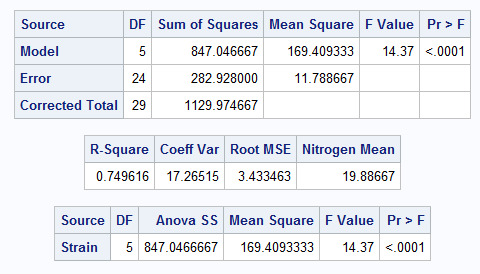
\includegraphics[scale=0.85]{cloveranova}
\end{flushleft}

\newpage

How do we check our assumptions? \\~\\
To investigate the constant variance assumption, we can look at side-by-side box plots or residual vs predicted plots.  A residual is the observed value minus the predicted value.  For the $ij^{th}$ observation the residual is
$$r_{ij}=obs-pred=y_{ij}-\bar{y}_{i\bullet}$$

\begin{wrapfigure}{r}{0.5\textwidth}
	\begin{center}
		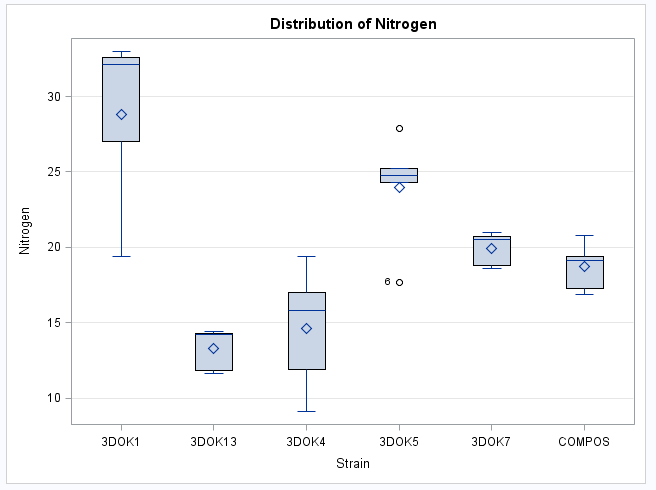
\includegraphics[scale=0.55]{cloveranova2}
  \end{center}
\end{wrapfigure}
~\\~\\
If the constant variance assumption is violated, one thing we might do is try a transformation of the data.  This will be looked at in ST 512.\\~\\~\\~\\
To check the normality, we look for a straight line in the qq-plot (or quantile vs residual plot) and also we hope to see a roughly normal looking histogram in the bottom left panel.  (Note: the transformation idea above may also solve some nonnormality issues.)\\~\\

	\begin{center}
	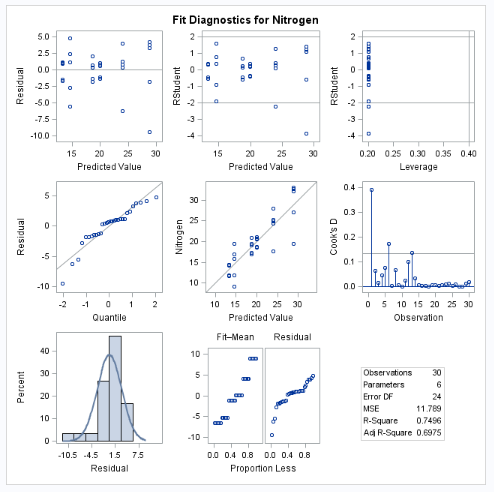
\includegraphics[scale=0.8]{cloveranova4}
  \end{center}

\newpage
~\\~\\~\\
If we reject $H_0$ and conclude that the treatment means differ, the next logical question to ask is which treatment means are the ones that differ.  \\~\\

To answer this question we usually look at all pairwise comparisons of treatment means.  That is, if we reject $H_0$, we would look at 
$$\mu_1-\mu_2~~~\mu_1-\mu_3~~~~~\cdots~~~~~\mu_1-\mu_t$$
$$\mu_2-\mu_3~~~~\cdots~~~~ \mu_{t-1}-\mu_{t}$$
to see which differ.\\~\\

Let's focus on $\mu_1-\mu_2$.  We get an estimator this quantity with the corresponding sample means
$$\hat{\mu}_{1}-\hat{\mu}_{2}=\bar{Y}_{1\bullet}-\bar{Y}_{2\bullet}$$~\\

The standard error of this quantity can be found by taking the square root of the variance (recall we assume our samples are independent so covariance is 0)
$$Var(\bar{Y}_{1\bullet}-\bar{Y}_{2\bullet}) = (1^2)Var(\bar{Y}_{1\bullet})+(-1)^2\bar{Y}_{2\bullet}+2(1)(-1)Cov(\bar{Y}_{1\bullet},\bar{Y}_{2\bullet})$$
$$=Var(Y_{1j})/n_1+Var(Y_{2j})/n_2 = \sigma^2/n_1+\sigma^2/n_2$$~\\

For a balanced design we have
$$Var(\bar{Y}_{1\bullet}-\bar{Y}_{2\bullet}) = \sigma^2(1/n+1/n) = 2\sigma^2/n$$
yielding a standard error of
$$SE(\bar{Y}_{1\bullet}-\bar{Y}_{2\bullet})=\sqrt{2\sigma^2/n}$$~\\

By the normality assumption on the data we then have a case similar to the two-sample t test with pooled variance!\\~\\
$$\bar{Y}_{1\bullet}-\bar{Y}_{2\bullet}\sim N(\mu_1-\mu_2,\sigma^2(1/n_1+1/n_2)) = N(\mu_1-\mu_2,2\sigma^2/n) $$~\\

We estimate $\sigma^2$ by the common pooled estimate (over all the samples, not just these two)
$$MS(E)=S^2_w=\frac{\sum_{i=1}^{t}\sum_{j=1}^{n}(Y_{ij}-\bar{Y}_{i\bullet})^2}{N-t}$$

\newpage


Thus, we can for a t-test for testing $H_0:\mu_1=\mu_2~~~vs~~~H_A:\mu_1\neq\mu_2$ using
$$T=\frac{\bar{Y}_{1\bullet}-\bar{Y}_{2\bullet}}{\sqrt{MS(E)(1/n_1+1/n_2)}}=\frac{\bar{Y}_{1\bullet}-\bar{Y}_{2\bullet}}{\sqrt{2MS(E)/n}}\sim t_{N-t}$$
and we can form a $(1-\alpha)100\%$ CI for $\mu_1-\mu_2$ using
$$\bar{Y}_{1\bullet}-\bar{Y}_{2\bullet}\pm t_{\alpha/2,N-t}\sqrt{MS(E)(1/n_1+1/n_2)}~~~or~~~\bar{Y}_{1\bullet}-\bar{Y}_{2\bullet}\pm t_{\alpha/2,N-t}\sqrt{2MS(E)/n}$$
and check if 0 is in the interval.\\~\\

An issue arises!  If we do this for all of the possible pairwise comparisons, we control the type I error rate for each test/interval, but by doing so many tests, the overall probability of making \textbf{at least one type I error} may be much more than $\alpha$.  This is known as the multiple comparison correction issue.  This will be taken up in ST 512.\\

\begin{center}
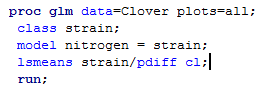
\includegraphics[scale=0.8]{cloverdiff0}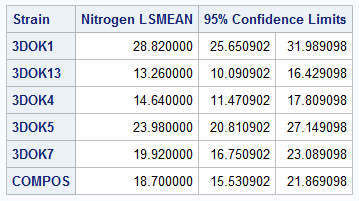
\includegraphics[scale=0.8]{cloverdiff1}\\
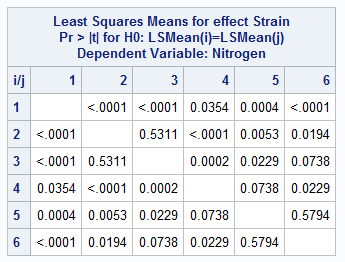
\includegraphics[scale=0.7]{cloverdiff2}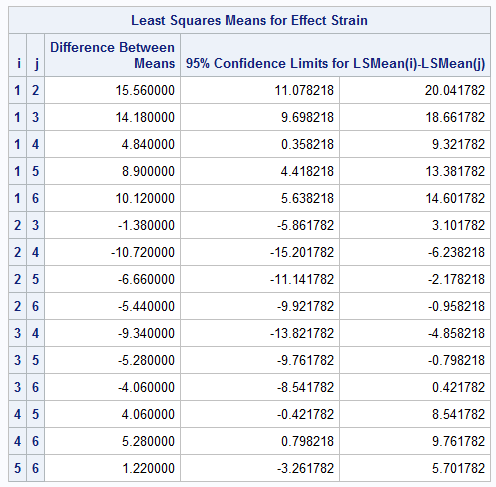
\includegraphics[scale=0.7]{cloverdiff3}
\end{center}

Multiple comparison correction needed!

